\documentclass[11pt]{article}
\usepackage[margin=1in]{geometry}
\usepackage{amsmath,amssymb}
\usepackage{graphicx}
\usepackage{booktabs}
\usepackage{url}
\usepackage[hidelinks]{hyperref}
% Generated by scripts/paper_numbers.py from committed results; do not edit by hand.
% Anchor check passed: confirmatory macros identical from verdict.json and endpoints.csv.
\newcommand{\ACobstViolPct}{89}
\newcommand{\ACrrViolPct}{85}
\newcommand{\AciHione}{\ensuremath{-4.85}}
\newcommand{\AciHithree}{\ensuremath{-43.04}}
\newcommand{\AciHitwo}{\ensuremath{-14.98}}
\newcommand{\AciLoone}{\ensuremath{-5.78}}
\newcommand{\AciLothree}{\ensuremath{-45.11}}
\newcommand{\AciLotwo}{\ensuremath{-16.49}}
\newcommand{\Adiffone}{\ensuremath{-5.30}}
\newcommand{\Adiffthree}{\ensuremath{-44.08}}
\newcommand{\Adifftwo}{\ensuremath{-15.72}}
\newcommand{\AfirstObstPeriod}{30}
\newcommand{\AfiveCount}{1}
\newcommand{\AfiveGap}{0.087}
\newcommand{\AfiveH}{\ensuremath{-0.00777}}
\newcommand{\AhoNegPct}{80}
\newcommand{\AlphaStar}{10}
\newcommand{\Apassone}{met}
\newcommand{\Apassthree}{met}
\newcommand{\Apasstwo}{met}
\newcommand{\Apone}{\ensuremath{2.6\times 10^{-144}}}
\newcommand{\Apthree}{\ensuremath{<10^{-300}}}
\newcommand{\Aptwo}{\ensuremath{<10^{-300}}}
\newcommand{\AucPooled}{0.96}
\newcommand{\Aupperone}{\ensuremath{-4.82}}
\newcommand{\Aupperthree}{\ensuremath{-42.95}}
\newcommand{\Auppertwo}{\ensuremath{-14.92}}
\newcommand{\BCobstViolPct}{4}
\newcommand{\BCrrViolPct}{36}
\newcommand{\BciHione}{5.27}
\newcommand{\BciHithree}{11.27}
\newcommand{\BciHitwo}{10.53}
\newcommand{\BciLoone}{4.35}
\newcommand{\BciLothree}{9.84}
\newcommand{\BciLotwo}{9.10}
\newcommand{\Blossone}{4.81}
\newcommand{\Blossthree}{10.56}
\newcommand{\Blosstwo}{9.81}
\newcommand{\Bpassone}{not met}
\newcommand{\Bpassthree}{not met}
\newcommand{\Bpasstwo}{not met}
\newcommand{\Bupperone}{5.31}
\newcommand{\Bupperthree}{11.33}
\newcommand{\Buppertwo}{10.59}
\newcommand{\CapBindMax}{8}
\newcommand{\CapBindMin}{1}
\newcommand{\CapMedMax}{0.78}
\newcommand{\CapMedMin}{0.72}
\newcommand{\CciHione}{0.0126}
\newcommand{\CciHithree}{0.0290}
\newcommand{\CciHitwo}{0.0212}
\newcommand{\CciLoone}{0.0108}
\newcommand{\CciLothree}{0.0266}
\newcommand{\CciLotwo}{0.0192}
\newcommand{\Celigone}{9{,}000}
\newcommand{\Celigthree}{9{,}000}
\newcommand{\Celigtwo}{9{,}000}
\newcommand{\Cexclone}{0}
\newcommand{\Cexclthree}{0}
\newcommand{\Cexcltwo}{0}
\newcommand{\Cincone}{0.0117}
\newcommand{\Cincthree}{0.0278}
\newcommand{\Cinctwo}{0.0202}
\newcommand{\Cnormone}{0.0126}
\newcommand{\Cnormthree}{0.0291}
\newcommand{\Cnormtwo}{0.0213}
\newcommand{\CollBmone}{0}
\newcommand{\CollBmthree}{0}
\newcommand{\CollBmtwo}{0}
\newcommand{\CollOffone}{483}
\newcommand{\CollOffthree}{4{,}319}
\newcommand{\CollOfftwo}{1{,}490}
\newcommand{\CollOnone}{0}
\newcommand{\CollOnthree}{0}
\newcommand{\CollOntwo}{0}
\newcommand{\Cpassone}{not met}
\newcommand{\Cpassthree}{not met}
\newcommand{\Cpasstwo}{not met}
\newcommand{\Cupperone}{0.0127}
\newcommand{\Cupperthree}{0.0291}
\newcommand{\Cuppertwo}{0.0213}
\newcommand{\FailOffone}{5.4}
\newcommand{\FailOffthree}{48.0}
\newcommand{\FailOfftwo}{16.6}
\newcommand{\FailOnone}{0.1}
\newcommand{\FailOnthree}{3.9}
\newcommand{\FailOntwo}{0.8}
\newcommand{\GapAmedCm}{3.3}
\newcommand{\GapBmedCm}{14.4}
\newcommand{\GoalBmone}{48.8}
\newcommand{\GoalBmthree}{19.3}
\newcommand{\GoalBmtwo}{53.5}
\newcommand{\GoalOffone}{54.7}
\newcommand{\GoalOffthree}{32.0}
\newcommand{\GoalOfftwo}{66.6}
\newcommand{\GoalOnone}{49.9}
\newcommand{\GoalOnthree}{21.5}
\newcommand{\GoalOntwo}{56.8}
\newcommand{\GroupA}{2{,}274}
\newcommand{\GroupAnb}{15}
\newcommand{\GroupAobst}{2{,}259}
\newcommand{\GroupAprime}{2{,}540}
\newcommand{\GroupB}{11{,}255}
\newcommand{\InfBmone}{0}
\newcommand{\InfBmthree}{0}
\newcommand{\InfBmtwo}{0}
\newcommand{\InfHdiffMax}{\ensuremath{4.3\times 10^{-8}}}
\newcommand{\InfNear}{410}
\newcommand{\InfOnone}{6}
\newcommand{\InfOnthree}{352}
\newcommand{\InfOntwo}{75}
\newcommand{\InfRepro}{433}
\newcommand{\InfRobots}{433}
\newcommand{\InfSlackMax}{\ensuremath{-8.4\times 10^{-9}}}
\newcommand{\InfSlackMin}{\ensuremath{-4.9\times 10^{-6}}}
\newcommand{\InfTotal}{433}
\newcommand{\OnBmGoalMax}{3.2}
\newcommand{\OnBmGoalMin}{1.0}
\newcommand{\OnMinusBmGoalone}{1.0}
\newcommand{\OnMinusBmGoalthree}{2.2}
\newcommand{\OnMinusBmGoaltwo}{3.2}
\newcommand{\PairsPerDensity}{9{,}000}
\newcommand{\RgrOffone}{94.6}
\newcommand{\RgrOffthree}{51.3}
\newcommand{\RgrOfftwo}{83.2}
\newcommand{\RgrOnone}{87.1}
\newcommand{\RgrOnthree}{35.0}
\newcommand{\RgrOntwo}{69.5}
\newcommand{\SelGoalfive}{1{,}936}
\newcommand{\SelGoalhalf}{0}
\newcommand{\SelGoalone}{255}
\newcommand{\SelGoalten}{2{,}224}
\newcommand{\SelGoaltwo}{1{,}184}
\newcommand{\SelInffive}{61}
\newcommand{\SelInfhalf}{1{,}251}
\newcommand{\SelInfone}{4}
\newcommand{\SelInften}{129}
\newcommand{\SelInftwo}{11}
\newcommand{\SelN}{5{,}400}
\newcommand{\TObmone}{51.2}
\newcommand{\TObmthree}{80.7}
\newcommand{\TObmtwo}{46.5}
\newcommand{\TOfi}{9{,}211}
\newcommand{\TOfiObst}{9{,}143}
\newcommand{\TOfiOffColl}{5{,}699}
\newcommand{\TOfiOffGoal}{2{,}274}
\newcommand{\TOfiPct}{61}
\newcommand{\TOng}{5{,}670}
\newcommand{\TOngOffTO}{5{,}362}
\newcommand{\TOngPct}{38}
\newcommand{\TOoffone}{39.9}
\newcommand{\TOoffthree}{20.0}
\newcommand{\TOofftwo}{16.9}
\newcommand{\TOonTotal}{15{,}038}
\newcommand{\TOonone}{50.1}
\newcommand{\TOonthree}{74.6}
\newcommand{\TOontwo}{42.4}
\newcommand{\ThrMatchObstFive}{43.1}
\newcommand{\ThrOffGoal}{51.1}
\newcommand{\ThrOnGoal}{42.7}
\newcommand{\ThrRetObstFive}{84.4}
\newcommand{\TrialsTotal}{27{,}000}
\newcommand{\Verdictone}{not shown useful}
\newcommand{\Verdictthree}{not shown useful}
\newcommand{\Verdicttwo}{not shown useful}
\newcommand{\Vp}{0.50}


\title{An Execution-Time CBF-QP Safety Filter on Frozen MAPPO Formation Policies:\\
A Pre-Specified Paired Evaluation in Simulation}
\author{Al Mahdi Sallam\\KFUPM}
\date{}

\begin{document}
\maketitle
\begin{center}
\fbox{\parbox{0.9\linewidth}{\centering\textbf{DRAFT - not for distribution; authorship and framing pending advisor review}}}
\end{center}

{\sloppy\paragraph{AI-assistance statement.} The code, analyses and this draft were produced with
substantial assistance from an AI coding assistant (Claude, Anthropic) under the author's direction.
Every number in the text is generated by committed scripts from committed result files
(\texttt{scripts/paper\_numbers.py}, \texttt{paper/numbers.tex}). The author is responsible for the content.\par}

\begin{abstract}
We evaluate whether an execution-time, decentralised control-barrier-function quadratic-programme
(CBF-QP) safety filter, placed between frozen multi-agent PPO (MAPPO) formation policies and a
simulated differential-drive team, is useful under criteria fixed before the test. Nine frozen
actors (three training seeds, three checkpoints each) were evaluated on reserved, previously
unused layouts with one, two and three obstacles (\PairsPerDensity{} paired trials per density),
with the filter off, the filter on at the gain $\alpha^\star=\AlphaStar$ selected on validation
layouts, and a brake comparator. The filter reduced the share of trials ending in collision or
infeasibility at every density (from \FailOffone\% to \FailOnone\%, \FailOfftwo\% to \FailOntwo\% and
\FailOffthree\% to \FailOnthree\%). Under the pre-set criteria it was nevertheless \emph{not shown
useful} at any density: the non-inferiority criteria for goal completion (margin five percentage
points) and for formation error over the common executed prefix (margin 0.01\,m) were not met.
Exploratory, post hoc analyses of the saved logs indicate that many filtered runs stalled in
front of obstacles on layouts the unfiltered policy completed or collided on, and that in all
\InfTotal{} infeasible trials the binding barrier row sat at its stand-off, consistent with
numerical sensitivity at $\alpha\Delta=1$. Claims cover these nine actors in this simulated
scenario only.
\end{abstract}

\section{Introduction}
Reinforcement-learning policies for multi-robot formations are commonly trained without safety
constraints \cite{brunke2022}, and a control-barrier-function (CBF) safety filter \cite{ames2019}
can be added at execution time without retraining. Whether such a filter is \emph{useful}, i.e.
reduces failures without an unacceptable loss of task completion or formation quality, is an
empirical question for a given policy family. This draft reports a pre-specified paired evaluation
of one such filter, a decentralised sampled-data CBF-QP, on frozen MAPPO actors in a VMAS
differential-drive formation-navigation scenario, followed by clearly labelled exploratory analyses
of why the pre-set criteria were not met.

\paragraph{Research question.} Does an execution-time CBF-QP filter, applied to frozen MAPPO
formation policies trained without it, reduce collisions, and at what cost in formation error,
goal completion and deadlock?

\paragraph{Motivating hypotheses (Stage~2).} The study was motivated by three hypotheses stated
in an earlier (Stage~2) submission, quoted here: ``H1: collisions fall. H2: formation error and
completion time rise, more so in denser layouts. H3: most failures under filtering come from
deadlock or infeasible steps rather than slower progress.'' Stage~2 defined deadlock as ``centroid
progress below a set distance over a set window'' (the protocol's stalled flag). These hypotheses
motivate the design; they do not extend the locked confirmatory claims, which are the three
criteria of Section~\ref{sec:design}. Section~\ref{sec:discussion} maps each hypothesis to the
evidence and states which evidence is confirmatory and which is exploratory.

\section{Related work}\label{sec:related}
Safe learning in robotics is surveyed in \cite{brunke2022} and control barrier functions in
\cite{ames2019}. Multi-agent approaches differ in when safety enters. Some learn the policy with
a CBF shield or a learned barrier certificate during training
\cite{cai2021,qin2021,zhang2025gcbf,zhang2025dgppo,deng2026}; some filter during both training and
execution \cite{choi2025,dawood2025}; and some filter at execution only, after training without
the filter: \cite{vinod2022} (centralised QP, linear and double-integrator agents).
Table~\ref{tab:related} summarises them. Here \emph{paired on/off} means that the same frozen
policy is evaluated with and without the filter on matched layouts; a comparison between separately
trained policies (a training ablation) does not count as paired in this sense. The table is
adapted from the Stage~2 submission and is provisional: its classifications were \emph{not
verified} against the papers in this revision.

Sampled-data CBF margins that account for inter-sample behaviour are studied in
\cite{singletary2020,breeden2022,tan_zocbf,liu_sacbf}; these margins are input-independent bounds
over the input set and do not depend on the applied command. Decentralised equal-split
(``half-responsibility'') constraints go back to \cite{wang2017,vandenberg2011}, and stopping as a
feasibility-preserving backup is used in \cite{chen2021}. The offset (barrier) point for unicycles
is used in \cite{emam2019}. Hidden assumptions in CBF safety claims are discussed in
\cite{kim2026}. Input-dependent inter-sample bounds used for trigger timing appear in
\cite{yang2019}. Interval estimates and per-seed reporting for RL evaluation are argued for in
\cite{agarwal2021}.

\begin{table}[t]
\centering\small
\caption{Related multi-agent studies (adapted from the Stage~2 submission; provisional, classifications
not verified against the papers). ``Paired on/off'' = the same frozen policy with and without the filter on
matched layouts.}
\label{tab:related}
\resizebox{\textwidth}{!}{%
\begin{tabular}{llll}
\toprule
Study & When safety is added & Paired on/off & Other outcomes\\
\midrule
Cai et al. \cite{cai2021} & CBF shield in training & No & reward\\
Qin et al. \cite{qin2021} & learned with controller & refinement only & safety rate, reward\\
GCBF+ \cite{zhang2025gcbf} & learned with controller & No & reach, success\\
DGPPO \cite{zhang2025dgppo} & learned with MARL policy & No & task performance, safety rate\\
Choi et al. \cite{choi2025} & CBVF filter in training and execution & unclear & conflicts, travel time, distance\\
Deng et al. \cite{deng2026} & learned after freezing & not shown & arrival rate\\
Dawood et al. \cite{dawood2025} & MPC filter in training & Yes (Stage 2); see note & success, time, formation, timeouts\\
Vinod et al. \cite{vinod2022} & QP filter at execution after training without it (centralised) & not stated here & not stated here\\
This study & CBF-QP after training & Yes & formation, completion, interventions, infeasibility, stalls\\
\bottomrule
\end{tabular}}
\par\smallskip\footnotesize Note: the methodology notes for this project record that \cite{dawood2025}
has no deployment-only baseline for a filter-unaware policy, so its on/off comparison may be a
training ablation rather than a paired evaluation in the sense above (not verified).
\end{table}

\section{System and filter}\label{sec:system}
\paragraph{Robots and task.} Three differential-drive robots with axle-centre pose $x=(x,y,\theta)$,
body disc of radius $R=0.10$\,m, and command $u=(v,\omega)$ in the box
$\mathcal U=\{-0.5\le v\le 0.5\ \mathrm{m/s},\ |\omega|\le 1\ \mathrm{rad/s}\}$ follow the unicycle model
\begin{equation}
\dot x = v\cos\theta,\qquad \dot y = v\sin\theta,\qquad \dot\theta=\omega ,
\end{equation}
with commands held over each control period $\Delta=0.1$\,s (zero-order hold). The team moves a
triangular formation (slot radius 0.30\,m) through a field of $K$ circular obstacles of radius
$R_o=0.20$\,m to a goal within a horizon of 400 periods. GOAL requires the centroid within 0.10\,m of
the goal and mean slot error within 0.10\,m; COLLISION is scored on the swept path and ends the trial;
an infeasible QP ends the trial as INFEASIBLE before any motion; otherwise the trial ends as TIMEOUT.

\paragraph{Offset point and barriers.} The filter constrains the point
$p=(x+\ell\cos\theta,\ y+\ell\sin\theta)$, $\ell=0.05$\,m, for which
\begin{equation}
\dot p = J(\theta)\,u,\qquad J(\theta)=\begin{bmatrix}\cos\theta & -\ell\sin\theta\\ \sin\theta & \ell\cos\theta\end{bmatrix},\qquad \det J=\ell ,
\end{equation}
so every barrier below has relative degree one in $(v,\omega)$. The barriers are
\begin{equation}
h_o=\|p-c\|^2-D_o^2,\quad D_o=R+\ell+R_o;\qquad h_{ij}=\|p_i-p_j\|^2-D_{rr}^2,\quad D_{rr}=2(R+\ell).
\end{equation}
Because $\|x-p\|=\ell$, the body disc lies inside the \emph{cover disc} of radius $R+\ell$ around
$p$, so $h\ge0$ implies physical separation. The converse does not hold: depending on the heading,
a robot whose body is a few centimetres from an obstacle can have $h_o<0$ (Fig.~\ref{fig:f0}).

\begin{figure}[t]\centering
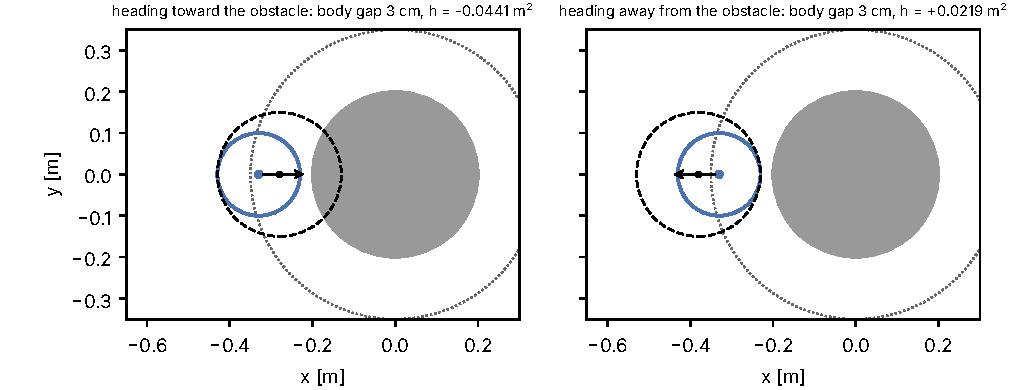
\includegraphics[width=0.95\linewidth]{figures/F0_cover_disc_schematic.pdf}
\caption{Analytic schematic (no data). Body disc (solid), axle centre, offset point $p$ and cover disc
of radius $R+\ell$ (dashed) next to an obstacle (grey) whose barrier boundary $\|p-c\|=D_o$ is dotted. With
the same 3\,cm body clearance, the cover barrier is negative when the robot heads toward the obstacle and
positive when it heads away.}\label{fig:f0}
\end{figure}

\paragraph{Sampled-data condition.} The implemented filter uses the following lemma with a
two-sided bound on $\ddot h$; only the lower bound is needed.

\emph{Lemma 1 (one-sided form).} Let $u$ be held on $[t_k,t_k+\Delta]$, $\ddot h\ge -M$ on that
interval with $M\ge0$, $\alpha\Delta\le 1$ and $h(t_k)\ge 0$. If
$\dot h(t_k)+\alpha h(t_k)\ge \delta=M\Delta/2$, then
$h(t_k+s)\ge (1-\alpha s)\,h(t_k)\ge 0$ for all $s\in[0,\Delta]$.

This is the second-order approach of \cite{breeden2022} (Theorem~3, stated there with the opposite
sign convention for $h$; $\gamma\le1$ corresponds to $\alpha\Delta\le1$). With
$V_p=\sqrt{\bar v^2+\ell^2\bar\omega^2}$ and $A_p=\bar\omega V_p$, the implemented margins use the
two-sided bounds of the design document,
\begin{equation}
\delta_o(d)=\tfrac{\Delta}{2}\big[2V_p^2+2(d+V_p\Delta)A_p\big],\qquad
\delta_{ij}(d)=\tfrac{\Delta}{2}\big[8V_p^2+4(d+2V_p\Delta)A_p\big],
\end{equation}
where $d$ is the current barrier-point distance. At $\alpha\Delta=1$ the lemma gives
$h(t_k+\Delta)\ge 0$ but no strictly positive endpoint bound (Section~\ref{sec:discussion}).

\paragraph{Equal split and the per-robot QP.} With $g_o=2J(\theta_i)^\top(p_i-c)$ and
$g_{ij}=2J(\theta_i)^\top(p_i-p_j)$, robot $i$ solves at every period
\begin{equation}
\begin{aligned}
\min_{u\in\mathcal U}\ & \tfrac12\|u-u_{\rm nom}\|^2\\
\text{s.t. }& g_o^\top u\ \ge -\alpha h_o+\delta_o(d) && \text{obstacles with } d\le 1.0\,\mathrm{m},\\
& g_{ij}^\top u\ \ge -\tfrac{\alpha}{2}h_{ij}+\tfrac12\delta_{ij}(d) && \text{neighbours with } d\le 1.5\,\mathrm{m},
\end{aligned}
\end{equation}
where $u_{\rm nom}$ is the frozen actor's deterministic command. Each robot takes half of every pair
condition (equal split); the two halves sum to the pair condition of Lemma~1 when both robots use the
same state. The two-variable QP is solved exactly by enumerating candidate points, with a feasibility
tolerance of $10^{-9}$ on normalised rows; there is no fallback, so an infeasible QP ends the trial.
The B-match comparator applies $(0,\omega_{\rm nom})$ whenever the clipped nominal command violates
one of these rows at the same gain; it is not a certified stop (the offset point rotates).

\section{Policy and training}\label{sec:policy}
\paragraph{Observation and reward.} Each robot observes, in its body frame: its slot error relative
to the centroid, the centroid-to-goal vector (norm-clipped at 2.0\,m), teammates' relative positions
and headings, the eight nearest obstacles within 2.0\,m (relative centre, surface gap, present flag)
and an agent one-hot. The per-period reward is
$10\cdot$(centroid progress toward the goal) $-1\cdot$(mean slot error) $-0.01\cdot$(control effort)
$-10\cdot$[collision] $-0.2\cdot\sum_{\rm pairs}\max(0,1-\text{clearance}/0.15\,\mathrm{m})$; a collision
ends the episode and a timeout is bootstrapped. The filter is never used in training.

\paragraph{MAPPO and curriculum.} A compact PyTorch MAPPO (shared Gaussian actor with tanh-bounded
mean, centralised critic, GAE with $\gamma=0.99$, $\lambda=0.95$, clip 0.2, 10 epochs, 16 minibatches,
learning rates $3\times10^{-4}$ actor and $10^{-3}$ critic, 384 parallel environments of 64 steps) was
trained with three seeds through a curriculum $K=0\to1\to2\to3\to(2,5,8)$ with stage budgets of 1, 2,
4, 4 and 8 million environment steps. The implementation was sanity-checked only on the stock VMAS
navigation task, where the deterministic policy reached \MappoNavSuccess\% success on 200 fixed
episodes (uniform random: \MappoNavRandom\%).

\paragraph{Checkpoints and gate history.} The nine actors are the early, middle and late checkpoints
of the final curriculum stage of each seed, fixed by an iteration rule (first saved checkpoint with
$r\ge\lceil n/3\rceil$, $r\ge\lceil 2n/3\rceil$, and $r=n$, with $n=326$ final-stage iterations). The
original pre-registered filter-off gate (pooled GOAL $\ge$ 50\% over $K=2,5,8$) was not met by any
checkpoint: the best pooled GOAL rate was \GateVoneBest\% (first configuration) and \GateVtwoBest\%
(curriculum). $K=5,8$ were therefore moved to stress cells and $K=1,2,3$ became the primary densities.
Table~\ref{tab:baseline} shows the filter-off baseline of the nine actors on validation layouts.

\begin{table}[t]
\centering\small
\caption{Filter-off baseline on validation layouts (200 per cell): GOAL / COLLISION / TIMEOUT (\%) per actor and
obstacle count $K$ (descriptive context; $K=4$ was an intermediate diagnostic).}
\label{tab:baseline}
\begin{tabular}{lcccccc}
\toprule
actor & $K=1$ & $K=2$ & $K=3$ & $K=4$ & $K=5$ & $K=8$\\
\midrule
\TabBaselineRows
\bottomrule
\end{tabular}
\end{table}

\section{Experimental design}\label{sec:design}
The protocol was locked by the author before any filter-on data with the frozen MAPPO actors
existed; the margins and decisions were chosen without advisor review
(Section~\ref{sec:disclosures}). Filter-on results did exist before the lock in two other forms:
engineering stress tests of the filter with random and adversarial stand-in controllers
(\EngStressTrials{} paired trials) and paired demonstration runs with an obstacle-blind stand-in
controller. Neither used the frozen MAPPO actors. The frozen-MAPPO development sweep on validation
layouts followed the lock, and the reserved final evaluation followed the gain selection.

The gain was selected on existing validation layouts from $\alpha\in\{0.5,1,2,5,10\}$\,s$^{-1}$ by the
highest pooled filter-on GOAL count over the nine actors and $K=1,2,3$ (ties: fewer INFEASIBLE, then the
larger gain). The final test used 1{,}000 reserved layouts per actor and density, each run with the
filter off, the filter on at $\alpha^\star$ and B-match at $\alpha^\star$. Usefulness at a density
required all of: (a) a one-sided exact McNemar reduction in COLLISION-or-INFEASIBLE; (b) GOAL loss
(off minus on) with one-sided 98.33\% upper bound (Newcombe method~10) at most 0.05; (c) the
equal-actor-weighted mean increase in formation error over the common executed prefix with
stratified bootstrap 98.33\% upper bound at most 0.01\,m; each one-sided at $0.05/3$. Per-seed and
per-actor results, episode length, TIMEOUT and the stalled flag were pre-declared as secondary and
descriptive.

\section{Results (confirmatory)}\label{sec:results}
\paragraph{Gain selection (development data).} Pooled filter-on GOAL counts over \SelN{} validation
trials were \SelGoalhalf, \SelGoalone, \SelGoaltwo, \SelGoalfive{} and \SelGoalten{} for
$\alpha=0.5,1,2,5,10$, with \SelInfhalf, \SelInfone, \SelInftwo, \SelInffive{} and \SelInften{}
INFEASIBLE outcomes, so $\alpha^\star=\AlphaStar$ (Fig.~\ref{fig:f1}).

\begin{table}[t]
\centering\small
\caption{Confirmatory results, filter on ($\alpha^\star=\AlphaStar$) versus filter off, nine actors
pooled, \PairsPerDensity{} pairs per density. Differences in percentage points (pp); one-sided bounds
at 98.33\%; 95\% intervals descriptive.}
\label{tab:conf}
\resizebox{\textwidth}{!}{%
\begin{tabular}{lccc}
\toprule
 & $K=1$ & $K=2$ & $K=3$\\
\midrule
COLLISION-or-INFEASIBLE, off $\to$ on (\%) & \FailOffone{} $\to$ \FailOnone & \FailOfftwo{} $\to$ \FailOntwo & \FailOffthree{} $\to$ \FailOnthree\\
(a) difference on$-$off [pp] & \Adiffone & \Adifftwo & \Adiffthree\\
\quad 98.33\% upper; 95\% CI & \Aupperone; [\AciLoone, \AciHione] & \Auppertwo; [\AciLotwo, \AciHitwo] & \Aupperthree; [\AciLothree, \AciHithree]\\
\quad one-sided exact $p$; criterion & \Apone; \Apassone & \Aptwo; \Apasstwo & \Apthree; \Apassthree\\
GOAL off / on (\%) & \GoalOffone{} / \GoalOnone & \GoalOfftwo{} / \GoalOntwo & \GoalOffthree{} / \GoalOnthree\\
(b) GOAL loss off$-$on [pp] & \Blossone & \Blosstwo & \Blossthree\\
\quad 98.33\% upper (margin 5); criterion & \Bupperone; \Bpassone & \Buppertwo; \Bpasstwo & \Bupperthree; \Bpassthree\\
(c) formation increase [m] & \Cincone & \Cinctwo & \Cincthree\\
\quad bootstrap 98.33\% upper (margin 0.01) & \Cupperone & \Cuppertwo & \Cupperthree\\
\quad normal cross-check; eligible / excluded & \Cnormone; \Celigone / \Cexclone & \Cnormtwo; \Celigtwo / \Cexcltwo & \Cnormthree; \Celigthree / \Cexclthree\\
\quad criterion & \Cpassone & \Cpasstwo & \Cpassthree\\
\midrule
Verdict & \Verdictone & \Verdicttwo & \Verdictthree\\
\bottomrule
\end{tabular}}
\end{table}

Table~\ref{tab:conf} gives the confirmatory results. Criterion (a) was met at every density;
(b) and (c) were met at none, so the filter was \emph{not shown useful under the pre-set
criteria} at $K=1,2,3$. With the filter on there were \CollOnone, \CollOntwo{} and
\CollOnthree{} collisions and \InfOnone, \InfOntwo{} and \InfOnthree{} INFEASIBLE trials;
TIMEOUT rose from \TOoffone\%, \TOofftwo\% and \TOoffthree\% to \TOonone\%, \TOontwo\% and
\TOonthree\% (Fig.~\ref{fig:f2}). B-match had \CollBmone, \CollBmtwo{} and \CollBmthree{} collisions
and \InfBmone, \InfBmtwo{} and \InfBmthree{} INFEASIBLE outcomes, and reached GOAL in \GoalBmone\%,
\GoalBmtwo\% and \GoalBmthree\% of trials; the filter reached GOAL \OnMinusBmGoalone,
\OnMinusBmGoaltwo{} and \OnMinusBmGoalthree{} percentage points more often (descriptive).

\paragraph{Per seed and per actor (pre-declared secondary, descriptive).} Table~\ref{tab:perseed}
gives the three locked endpoints per training seed with 95\% intervals; no test or verdict is made
per seed, and a pooled result does not establish usefulness, or its absence, for each seed or actor.
Per-actor GOAL losses vary widely (Fig.~\ref{fig:f3}).

\begin{table}[t]
\centering\small
\caption{Locked endpoints per training seed (pre-declared secondary, descriptive; three actors and 3{,}000
pairs per row; 95\% intervals; no tests).}
\label{tab:perseed}
\resizebox{\textwidth}{!}{%
\begin{tabular}{cccccc}
\toprule
seed & $K$ & COLLISION-or-INFEASIBLE off $\to$ on (\%) & (a) difference [pp] & (b) GOAL loss [pp] & (c) formation increase [m]\\
\midrule
\TabPerSeedRows
\bottomrule
\end{tabular}}
\end{table}

\paragraph{Time to goal (pre-declared episode-length endpoint; exploratory, post hoc joint-success
analysis).} In pairs where both arms reached GOAL, Table~\ref{tab:ttg} compares executed periods to
GOAL (test arm minus filter off; positive = slower). The equal-actor mean weights the nine actors
equally; the median, Hodges--Lehmann estimate and Wilcoxon test are pair-weighted. Conditioning on
joint success selects the easier layouts and does not estimate the overall completion-time cost.

\begin{table}[t]
\centering\small
\caption{Time to goal in joint-success pairs (periods of 0.1\,s; test arm minus filter off; pre-declared
episode-length endpoint, exploratory joint-success analysis).}
\label{tab:ttg}
\resizebox{\textwidth}{!}{%
\begin{tabular}{lcccccccc}
\toprule
arm & $K$ & pairs & fewest per actor & equal-actor mean & median & HL & slower (\%) & Wilcoxon $p$\\
\midrule
\TabTtgRows
\bottomrule
\end{tabular}}
\end{table}

\paragraph{Validation versus final test (exploratory, post hoc).} Table~\ref{tab:valtest} sets the
development-sweep estimates at $\alpha=10$ (validation layouts, used for gain selection) beside the
final-test estimates.

\begin{table}[t]
\centering\small
\caption{Estimates at $\alpha=10$ on validation layouts (development data) and on the reserved final test
(exploratory, post hoc comparison; 95\% intervals).}
\label{tab:valtest}
\resizebox{\textwidth}{!}{%
\begin{tabular}{ccccccc}
\toprule
$K$ & data & pairs & fail off $\to$ on (\%) & GOAL off $\to$ on (\%) & GOAL loss [pp] & formation increase [m]\\
\midrule
\TabValTestRows
\bottomrule
\end{tabular}}
\end{table}

\paragraph{Stress cells (exploratory, post hoc, descriptive).} The development sweep also ran the
diagnostic and stress densities $K=4,5,8$ on validation layouts (Table~\ref{tab:stress}). They were not
part of the final test and did not affect gain selection.

\begin{table}[t]
\centering\small
\caption{Stress cells on validation layouts at $\alpha=10$ (outcome shares in \%; exploratory, post hoc,
descriptive; not part of the final test).}
\label{tab:stress}
\begin{tabular}{llccccc}
\toprule
$K$ & arm & trials & GOAL & COLLISION & INFEASIBLE & TIMEOUT\\
\midrule
\TabStressRows
\bottomrule
\end{tabular}
\end{table}

\begin{figure}[t]\centering
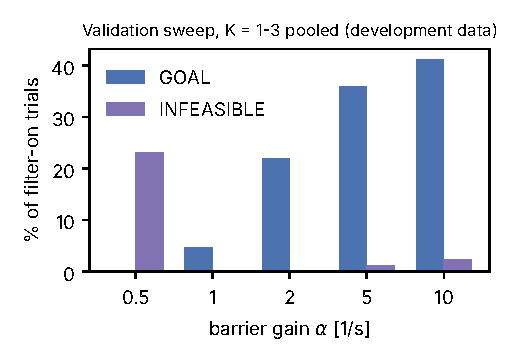
\includegraphics[width=0.48\linewidth]{figures/F1_validation_sweep.pdf}
\caption{Validation sweep (development data): filter-on GOAL and INFEASIBLE share per gain, $K=1$--3 pooled.}\label{fig:f1}
\end{figure}
\begin{figure}[t]\centering
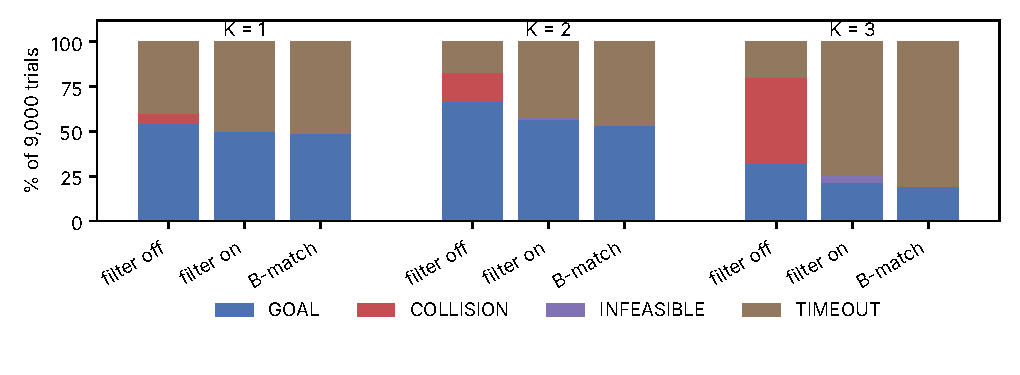
\includegraphics[width=0.95\linewidth]{figures/F2_final_outcomes.pdf}
\caption{Final-test outcome shares per density for filter off, filter on ($\alpha^\star$) and B-match.}\label{fig:f2}
\end{figure}
\begin{figure}[t]\centering
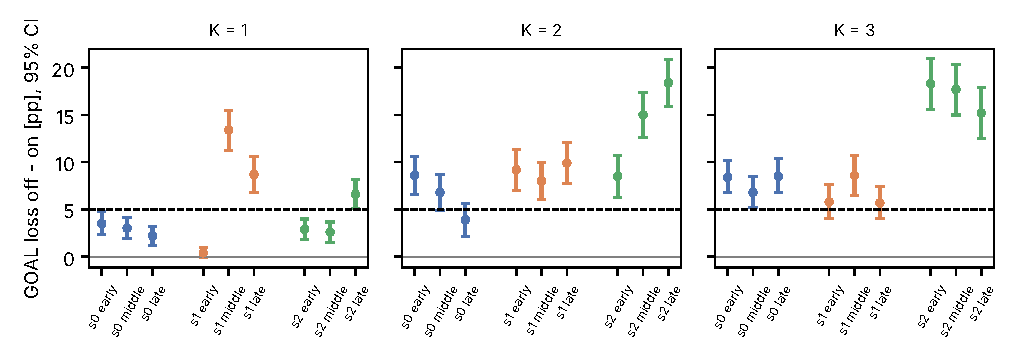
\includegraphics[width=0.95\linewidth]{figures/F3_per_actor_goal_loss.pdf}
\caption{Per-actor GOAL loss (off minus on) with descriptive 95\% Newcombe intervals, grouped by
training seed; dashed line: the 5\,pp margin of the pooled criterion (b).}\label{fig:f3}
\end{figure}

\section{Exploratory mechanism analysis (exploratory, post hoc)}\label{sec:mechanism}
\emph{Everything in this section is exploratory and post hoc: categories, thresholds, groups and the
example were chosen after the confirmatory results were known, the analyses read only saved logs,
and they support no causal or confirmatory claim.}

\paragraph{Stall classes.} Of \TOonTotal{} filter-on TIMEOUTs, \TOfi{} (\TOfiPct\%) were classified
as filter-induced stalls (the clipped nominal command violated an enabled barrier row in at least
half of the last 50 periods), \TOfiObst{} of them involving obstacle rows; on the same layouts the
unfiltered run collided in \TOfiOffColl{} and reached GOAL in \TOfiOffGoal{} cases. Another \TOng{}
(\TOngPct\%) were near-goal parking stalls, \TOngOffTO{} of them on layouts where the unfiltered run
also timed out.

\paragraph{Groups A and B.} Group A (\GroupA{} pairs: unfiltered GOAL, filtered filter-induced
stall; \GroupAobst{} obstacle-labelled, \GroupAnb{} neighbour-only) and group B (\GroupB{} pairs:
both GOAL) were selected by observed outcome. The unfiltered runs of group A came closer to
obstacles (median sampled minimum surface clearance \GapAmedCm\,cm, group A only) than those of
group B (\GapBmedCm\,cm; Fig.~\ref{fig:f4}). Their applied commands violated at least one filter
obstacle row in \ACobstViolPct\% (A) versus \BCobstViolPct\% (B) of runs, and a robot-pair row in
\ACrrViolPct\% versus \BCrrViolPct\%.

\paragraph{Example (exploratory, post hoc).} Fig.~\ref{fig:f6} shows one group-A pair, chosen by a
rule fixed before plotting: the pair whose unfiltered minimum sampled obstacle clearance is closest to
the unrounded group-A median (\ExMedCm\,cm), ties by actor index, density and trial. The rule selected
actor \ExActor, $K=\ExK$, trial \ExTrial{} (clearance \ExGapCm\,cm). The unfiltered run reached GOAL
after \ExOffT{} periods with its closest approach at period \ExCaState; the filtered run's centroid
stalled from period \ExStallState. At that instant, robot \ExRobot{} (the robot with the smallest
obstacle cover barrier, $h=\ExCoverH$\,m$^2$, body clearance \ExCoverGapCm\,cm) is shown with its
cover disc. This is a geometric selection: it does not show that this robot or constraint caused the
stall, and a centroid stall does not mean that every robot stopped.

\paragraph{Clearance thresholds.} Of all trials, \ThrOffGoal\% reached GOAL unfiltered, and
\ThrMatchObstFive\% did so while keeping a sampled minimum obstacle clearance of at least 5\,cm,
against a filter-on GOAL rate of \ThrOnGoal\% on the same layouts (Fig.~\ref{fig:f5}). This
describes how close the unfiltered runs came to obstacles; it does not measure what a buffer or
any filter would cost. Among unfiltered GOAL trials the descriptive AUC of the unfiltered minimum
obstacle clearance for ``filtered run did not reach GOAL'' was \AucPooled.

\paragraph{Infeasibility.} All \InfTotal{} INFEASIBLE trials were reproduced (\InfRepro{} of
\InfTotal) by the unchanged filter code at the saved states in an earlier audit. In every case the
binding row's barrier value was within \InfHdiffMax{}\,m$^2$ of its stand-off $h^\star=\delta/\alpha$
and the zero command violated it by between \InfSlackMax{} and \InfSlackMin{} (normalised);
\InfNear{} of \InfRobots{} met a pre-declared near-boundary diagnostic. This is consistent with
numerical sensitivity near the boundary, not proof of the cause.

\paragraph{Transit.} During formation transit the equal-split cap on a robot's closing speed toward
a neighbour had median \CapMedMin--\CapMedMax\,m/s, above the largest barrier-point speed
\Vp\,m/s, and bound in \CapBindMin--\CapBindMax\% of moving closing periods.

\begin{figure}[t]\centering
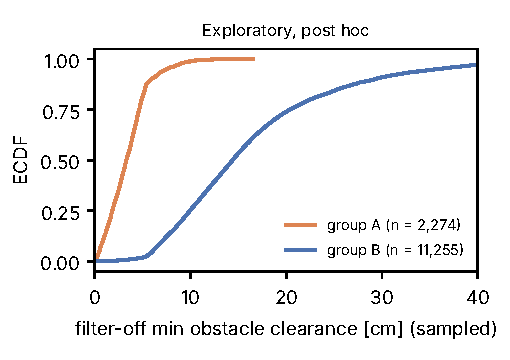
\includegraphics[width=0.48\linewidth]{figures/F4_clearance_groups.pdf}\hfill
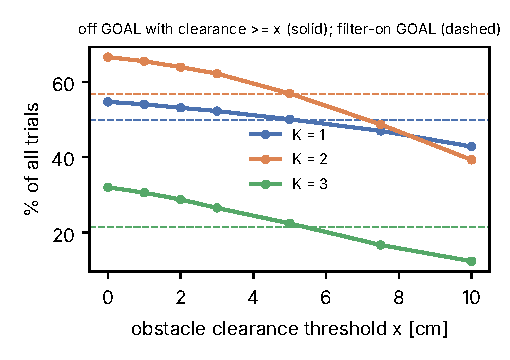
\includegraphics[width=0.48\linewidth]{figures/F5_matched_denominator.pdf}
\caption{Exploratory, post hoc. Left (F4): unfiltered minimum obstacle clearance (sampled), group A
vs group B. Right (F5): share of all trials that reached GOAL unfiltered with clearance at least
$x$, per density, with the filter-on GOAL rate (dashed).}\label{fig:f4}\label{fig:f5}
\end{figure}
\begin{figure}[t]\centering
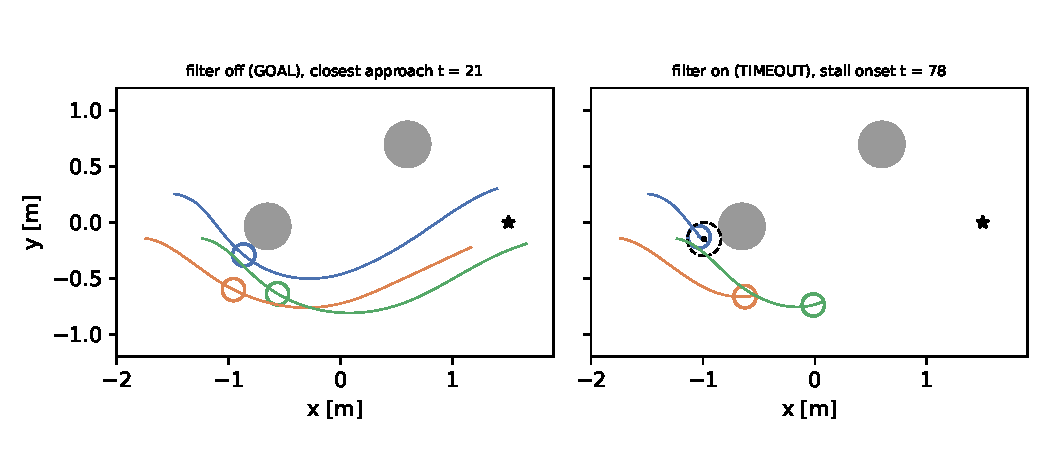
\includegraphics[width=0.95\linewidth]{figures/F6_example_trajectory.pdf}
\caption{Exploratory, post hoc example. Selection rule (fixed before plotting): among group-A pairs, the pair
whose filter-off minimum sampled obstacle clearance is closest to the unrounded group-A median; ties by actor
index, density, then trial. Left: filter off, bodies at the closest-approach instant. Right: filter on,
bodies at stall onset (first state from which the centroid stays within 0.05\,m of its final position), with
the cover disc (dashed, radius $R+\ell$) of the robot with the smallest obstacle barrier at that instant (ties by
robot index). Star: goal. Geometric selection only; not evidence of cause.}\label{fig:f6}
\end{figure}

\section{Discussion}\label{sec:discussion}
\paragraph{Hypotheses and evidence.}
\emph{H1 (collisions fall).} Supported for these actors: with the filter on there were \CollOnone,
\CollOntwo{} and \CollOnthree{} collisions against \CollOffone, \CollOfftwo{} and \CollOffthree{}
with the filter off (descriptive counts). The confirmatory endpoint is the composite
COLLISION-or-INFEASIBLE, whose reduction met criterion (a) at every density (Table~\ref{tab:conf});
collision counts alone were not a confirmatory endpoint.
\emph{H2 (formation error and completion time rise, more so in denser layouts).} The common-prefix
formation increase was \Cincone, \Cinctwo{} and \Cincthree\,m at $K=1,2,3$ and exceeded the
non-inferiority margin at every density (confirmatory, criterion (c)). The estimates increase with
density, but no density trend was tested, so the ``more so in denser layouts'' part is not
established. Completion fell (GOAL loss, criterion (b)); in joint-success pairs the time to goal
changed little (equal-actor mean \TtgEqOnone, \TtgEqOntwo{} and \TtgEqOnthree{} periods;
Table~\ref{tab:ttg}), and this conditional analysis does not estimate the completion-time cost.
\emph{H3 (failures under filtering come from deadlock or infeasible steps rather than slower
progress).} Of the \HthreeNongoalAll{} filter-on trials that did not reach GOAL, \HthreeShareAll\%
ended INFEASIBLE or as TIMEOUT with the protocol's stalled flag, and \HthreeMovingAll{} were TIMEOUTs
still progressing at the horizon (stalled flag pre-declared as secondary, descriptive). The split of
stalls into filter-induced and parking stalls is exploratory (Section~\ref{sec:mechanism}).

\paragraph{Collisions versus stalls.} With the filter on there were no collisions (\CollOnone,
\CollOntwo{} and \CollOnthree{} at $K=1,2,3$; the remaining failures were INFEASIBLE;
Table~\ref{tab:conf}); in the exploratory classification most filtered timeouts were stalls with
active obstacle rows, mostly on layouts where the unfiltered run collided or reached GOAL. We read
this as a description of where the lost completions occurred, not as a causal attribution. The
completions lost in group A involved unfiltered runs that passed close to obstacles (median
\GapAmedCm\,cm, group A only; Fig.~\ref{fig:f4}). The filter reached GOAL
\OnBmGoalMin--\OnBmGoalMax{} percentage points more often than B-match on the same layouts, with
more INFEASIBLE outcomes.

\paragraph{Gain at the lemma boundary.} The selected gain gives $\alpha^\star\Delta=1$. At
$\alpha^\star\Delta=1$, the lemma provides no strictly positive endpoint lower bound from the initial
barrier alone. Numerical robustness requires separate analysis. The infeasibility audit found the
recorded infeasible states consistent with numerical sensitivity near this boundary.

\paragraph{Predictions.} A methodology report written before the validation sweep, but committed to the
repository only after the final test (\texttt{docs/methodology/README.md}), predicted that the
selected gain would lie in $[5,10]$ and that small gains would conflict with holding the formation;
the sweep selected $\alpha^\star=\AlphaStar$ and gave \SelGoalhalf{} filter-on GOAL outcomes with
\SelInfhalf{} INFEASIBLE at $\alpha=0.5$ (Fig.~\ref{fig:f1}). Because of the commit order these are
documented, not pre-registered, predictions.

\paragraph{Remark (ZR).} For these offset-point barriers the second-order sampled-data margin can be
evaluated at the held command and written as two affine rows per barrier, which makes the zero
command admissible whenever $h\ge 0$ in exact arithmetic (design document, Section~4a). Its
ingredients are existing ideas \cite{breeden2022,vandenberg2011,chen2021}, the inclusion of
admissible sets is non-strict, and the property does not survive float32 rounding without a
separate tolerance rule; it was not implemented or evaluated here.

\paragraph{Practical implications (suggestions, each tied to a result; not findings).}
(i) Assess numerical robustness at the boundary gain; investigate gains strictly below the boundary or
an explicit tolerance rule in a separately designed follow-up (infeasibility audit). This is not
evidence that a lower gain would perform better: in the development sweep lower gains reached GOAL
less often (Fig.~\ref{fig:f1}).
(ii) Inspect the nominal policy's clearance distribution before deploying a filter: in the exploratory
analysis the unfiltered minimum obstacle clearance separated pairs that lost completion under the
filter (AUC \AucPooled).
(iii) Include a brake baseline: B-match came within \OnBmGoalMin--\OnBmGoalMax{} GOAL points of the
filter with no collisions or INFEASIBLE outcomes.
(iv) The small unfiltered clearances in group A suggest clearance-aware or filter-aware training as a
direction (exploratory).

\section{Limitations}
The study uses one simulated scenario, nine fixed actors from one custom MAPPO implementation,
three obstacle densities and one gain. Validation layouts were reused for gain tuning. The
formation criterion covers the common executed prefix only. Time to goal is analysed only in
joint-success pairs. Safety statements are numerical under the design-document assumptions, not a
continuous-time proof. The exploratory analyses are selected by observed outcome and descriptive.
The related-work classifications are provisional and were not verified against the papers.

\section{Future work}
Sensing noise or delay would test whether the unfiltered small-clearance passes stay collision-free.
Clearance-aware or filter-aware retraining, and a gain strictly below the boundary or an explicit
tolerance rule, are candidate follow-ups. Any such study would use the reserved, unused
5{,}000{,}000--5{,}999{,}999 layout block under its own locked protocol and disclose which of the
present post-test findings informed it.

\section{Reproducibility}
{\sloppy Code, configuration, saved logs and analyses are in \url{https://github.com/mahdisallam860/cbf-marl-filter-study}
(branch \texttt{claude/elegant-hopper-v8jxlv}). Protocol lock: commit \texttt{9baf6d7}; selected gain:
\texttt{4fffe62}; final test: \texttt{e23f8c3} (per-step logs \texttt{41ae3d4}); mechanism analyses:
\texttt{df78812}, \texttt{c2e331a}. Layout seeds: validation $2{,}000{,}000+K$; final test
$4{,}000{,}000+1{,}000p+K$ for actor index $p$; the block $5{,}000{,}000$--$5{,}999{,}999$ is reserved and
unused. The per-step logs of every final-test trial (poses, raw, clipped and applied commands,
interventions, brake activations) are committed, so all analyses here can be repeated without
re-running trials.\par}

\section{Mandatory disclosures}\label{sec:disclosures}
\begin{itemize}
\item The margins and protocol decisions were chosen by the author without advisor review; advisor agreement has not been obtained.
\item The protocol was locked before any filter-on data with the frozen MAPPO actors existed, but after engineering stress tests with random and adversarial stand-in controllers and demonstration runs with an obstacle-blind stand-in controller (the locked document's wording ``before any filter-on data existed'' is corrected here).
\item Filter-off validation results had been seen before the protocol was locked.
\item The checkpoint rule was committed before the Phase~1 evaluation but after earlier validation results were seen.
\item The validation layouts were reused as development data for gain tuning.
\item The methodology report was committed after the final test.
\item The mechanism categories were chosen after the confirmatory results were known.
\item The post-test decision rule was not committed before the mechanism results were read.
\item One of the \TrialsTotal{} final-test trials (s2\_early, $K=3$, trial 646) started with a negative obstacle cover barrier ($h=\AfiveH$\,m$^2$, body clearance \AfiveGap\,m), an exception to assumption A5; it is kept in all confirmatory numbers.
\item Claims cover these nine fixed actors in this simulated scenario only.
\item Safety statements are numerical under the design-document assumptions (A1--A9), not a continuous-time proof.
\item The MAPPO implementation is custom and was sanity-checked only on the stock VMAS navigation task.
\end{itemize}

\section{Conclusion}
Under the pre-set criteria, the execution-time CBF-QP filter at $\alpha^\star=\AlphaStar$ was not
shown useful for these nine frozen MAPPO actors at any of the three densities: it reduced
collision-or-infeasible failures but did not meet the non-inferiority criteria for goal completion
and common-prefix formation error.

\begin{thebibliography}{99}
\bibitem{brunke2022} L.~Brunke, M.~Greeff, A.~W.~Hall, Z.~Yuan, S.~Zhou, J.~Panerati, A.~P.~Schoellig, ``Safe learning in robotics: From learning-based control to safe reinforcement learning,'' \emph{Annual Review of Control, Robotics, and Autonomous Systems}, vol.~5, pp.~411--444, 2022, doi:10.1146/annurev-control-042920-020211.
\bibitem{ames2019} A.~D.~Ames, S.~Coogan, M.~Egerstedt, G.~Notomista, K.~Sreenath, P.~Tabuada, ``Control barrier functions: Theory and applications,'' Proc. 18th European Control Conference (ECC), 2019, pp.~3420--3431, doi:10.23919/ECC.2019.8796030.
\bibitem{wang2017} L.~Wang, A.~D.~Ames, M.~Egerstedt, ``Safety barrier certificates for collisions-free multirobot systems,'' \emph{IEEE Transactions on Robotics}, vol.~33, no.~3, pp.~661--674, 2017, doi:10.1109/TRO.2017.2659727.
\bibitem{deng2026} Z.~Deng, Q.~Li, M.~Zhang, W.~Chen, ``Safe multi-agent reinforcement learning through neural graph control barrier functions,'' Proc. AAMAS 2026, pp.~3232--3234, extended abstract, doi:10.65109/KRTJ4225.
\bibitem{dawood2025} M.~Dawood, S.~Pan, N.~Dengler, S.~Zhou, A.~P.~Schoellig, M.~Bennewitz, ``Safe multi-agent reinforcement learning for behavior-based cooperative navigation,'' \emph{IEEE Robotics and Automation Letters}, vol.~10, no.~6, pp.~6256--6263, 2025, doi:10.1109/LRA.2025.3560830.
\bibitem{cai2021} Z.~Cai, H.~Cao, W.~Lu, L.~Zhang, H.~Xiong, ``Safe multi-agent reinforcement learning through decentralized multiple control barrier functions,'' arXiv:2103.12553, 2021.
\bibitem{qin2021} Z.~Qin, K.~Zhang, Y.~Chen, J.~Chen, C.~Fan, ``Learning safe multi-agent control with decentralized neural barrier certificates,'' ICLR 2021, arXiv:2101.05436.
\bibitem{zhang2025dgppo} S.~Zhang, O.~So, M.~Black, C.~Fan, ``Discrete GCBF proximal policy optimization for multi-agent safe optimal control,'' ICLR 2025, arXiv:2502.03640.
\bibitem{choi2025} J.~J.~Choi, J.~J.~Aloor, J.~Li, M.~G.~Mendoza, H.~Balakrishnan, C.~Tomlin, ``Resolving conflicting constraints in multi-agent reinforcement learning with layered safety,'' Robotics: Science and Systems (RSS), 2025, doi:10.15607/RSS.2025.XXI.094.
\bibitem{zhang2025gcbf} S.~Zhang, O.~So, K.~Garg, C.~Fan, ``GCBF+: A neural graph control barrier function framework for distributed safe multiagent control,'' \emph{IEEE Transactions on Robotics}, vol.~41, pp.~1533--1552, 2025, doi:10.1109/TRO.2025.3530348.
\bibitem{agarwal2021} R.~Agarwal, M.~Schwarzer, P.~S.~Castro, A.~Courville, M.~G.~Bellemare, ``Deep reinforcement learning at the edge of the statistical precipice,'' NeurIPS 2021, vol.~34, pp.~29304--29320, arXiv:2108.13264.
\bibitem{vinod2022} Vinod et al., ``Safe multi-agent motion planning via filtered reinforcement learning,'' ICRA 2022 (MERL TR2022-053). \url{https://www.merl.com/publications/docs/TR2022-053.pdf}
\bibitem{singletary2020} Singletary, Chen, Ames, ``Control barrier functions for sampled-data systems with input delays,'' CDC 2020. \url{https://arxiv.org/pdf/2005.06418}
\bibitem{breeden2022} J.~Breeden, K.~Garg, D.~Panagou, ``Control barrier functions in sampled-data systems,'' \emph{IEEE Control Systems Letters}, doi:10.1109/LCSYS.2021.3076127. \url{https://arxiv.org/abs/2103.03677} (Theorem~3, second-order approach; checked against arXiv v2 on 2026-10-26; the paper uses the opposite sign convention for $h$)
\bibitem{tan_zocbf} Tan, Da\c{s}, Ames, Burdick (ZOCBF). \url{https://arxiv.org/html/2411.17079v2}
\bibitem{liu_sacbf} Liu, Xiao, Belta (SACBF), arXiv 2511.11897 v2. \url{https://arxiv.org/html/2511.11897v2}
\bibitem{vandenberg2011} van den Berg et al., 2011 (ORCA). \url{https://ics-websites.science.uu.nl/docs/vakken/mcrws/papers_new/van\%20den\%20Berg\%20et\%20al\%20-\%202011\%20-\%20Reciprocal\%20n-body\%20collision\%20avoidance.pdf}
\bibitem{chen2021} Chen, Singletary, Ames, IEEE L-CSS 2021. \url{https://par.nsf.gov/servlets/purl/10281485}
\bibitem{emam2019} Emam et al., CDC 2019. \url{https://arxiv.org/pdf/1909.02966}
\bibitem{kim2026} Kim, arXiv 2603.06954. \url{https://arxiv.org/html/2603.06954v1}
\bibitem{yang2019} Yang, Belta, Tron, ACC 2019. \url{https://arxiv.org/pdf/1903.03692}
\end{thebibliography}
\end{document}
